\begin{figure}[htbp]
    \centering
    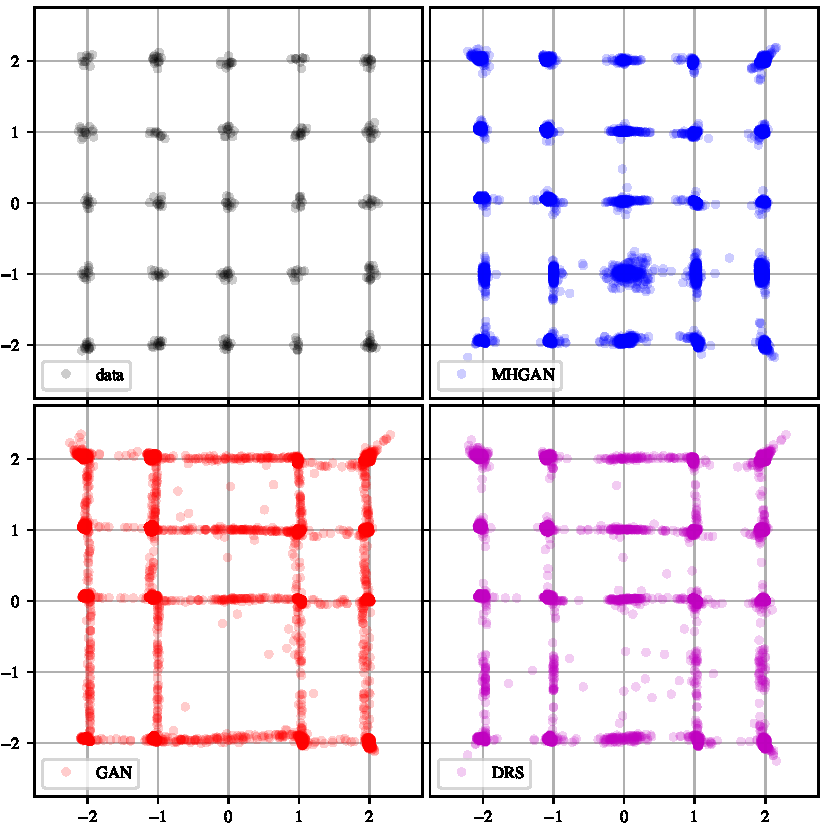
\includegraphics[scale=1.0]{figures/mog_example_30.pdf}
    \caption{{\small
    Data in the 25 Gaussians example (upper-left)\@.
    The other GAN setups are shown in the other figures.
    The MH-GAN corrects areas of mis-assigned mass in the original GAN\@.
    DRS appears visually closer to the original GAN than the data, whereas the MH-GAN appears closer to the actual data.
    }}
    \label{fig:mog_example}
\end{figure}

